% ============================================================================
%  Research Objective 3 — Monte-Carlo Probability Estimation
%  Replaces prior preliminary version; integrates new pipeline & diagnostics
% ============================================================================
\section{Research Objective 3: Develop data-parallel Monte Carlo algorithms for probability estimation}

% ----------------------------------------------------------------------------
%  Title Frame
% ----------------------------------------------------------------------------
\begin{frame}
  \Large\centering\textbf{Research Objective 3}\\[6pt]
  \large Develop data-parallel Monte-Carlo methods for estimating probabilities on unified PDAGs
\end{frame}

% ----------------------------------------------------------------------------
%  Bridge: From Boolean Evaluation to Probabilistic Inference
% ----------------------------------------------------------------------------
\begin{frame}{Bridging Boolean Evaluation and Probabilistic Inference}
  \begin{itemize}
    \item Previous objective delivered \emph{bit-parallel gate kernels} that evaluate a PDAG layer in $\mathcal{O}(1)$ machine words.
    \item To quantify \alert{risk}, we must attach \emph{probability distributions} to the PDAG leaves and propagate forward.
    \item Strategy: embed a Monte-Carlo engine that
          \begin{enumerate}
            \item draws bit-packed Bernoulli samples for \textbf{all} basic events, and
            \item reuses the same gate kernels to evaluate each random draw.
          \end{enumerate}
    \item One kernel pipeline therefore suffices for \textbf{both} deterministic logic and stochastic sampling.
  \end{itemize}
\end{frame}

\subsection{Back to Working Example: One Initiating Event, Three Fault Trees, Six Basic Events, Five End States}
\begin{frame}
  \begin{columns}
    \column{0.66\textwidth}
      \includesvg[height=\textheight]{1_concepts/dag_pass_3.svg} % Replace with your image file
     \column{0.33\textwidth}
      \includesvg[width=\linewidth]{1_concepts/pra-model.svg} % Replace with your image file
  \end{columns}  
\end{frame}

% ----------------------------------------------------------------------------
%  End-to-End Sampling Pipeline
% ----------------------------------------------------------------------------
\begin{frame}{End-to-End Sampling Pipeline (one iteration)}
  \begin{columns}
    \column{0.6\textwidth}
      \includesvg[height=0.9\textheight]{1_concepts/dag_pass_3.svg} % Replace with your image file
     \column{0.4\textwidth}
  \tiny   
  \begin{enumerate}[<+->]
    \item \textbf{Basic-Event Kernel:} generate random draws.
    \item \textbf{Gate Kernels:} evaluate PDAG layers using hardware-native logic primitives.
    \item \textbf{Tally Kernel:} count number of ones, update counters, compute estimates.
  \end{enumerate}
  \end{columns}  
\end{frame}

% ----------------------------------------------------------------------------
%  Monte-Carlo Algorithm Recap (keeps most of prior text)
% ----------------------------------------------------------------------------
\subsection{MC Sampling Theory}

\begin{frame}{Monte-Carlo Sampling over PDAGs}
  \small
  \begin{enumerate}
    \item Draw $\mathbf{x}^{(i)}\sim\prod_{b\in\mathcal{B}}\text{Bernoulli}\bigl(p_b\bigr)$ in \textbf{bit-packed} form.
    \item Evaluate the Boolean function $F\colon\{0,1\}^{|\mathcal{B}|}\!\to\!\{0,1\}$ (root node) using the gate kernels.
    \item Record $Y^{(i)} \!=\! F\bigl(\mathbf{x}^{(i)}\bigr)$ \;(failure indicator).
  \end{enumerate}
  After $N$ iterations
  \[\widehat{P}_N = \frac1N\sum_{i=1}^N Y^{(i)},\qquad \operatorname{SE}(\widehat P_N)=\sqrt{\frac{\widehat P_N(1-\widehat P_N)}{N}}.\]
  Error shrinks as $\mathcal{O}\!\bigl(N^{-1/2}\bigr)$; variance-reduction extensions discussed shortly.
\end{frame}


% ----------------------------------------------------------------------------
%  Basic-Event Sampling Kernel
% ----------------------------------------------------------------------------
\begin{frame}{Basic-Event Sampling Kernel}
\begin{columns}
  \column{0.7\textwidth}
  \footnotesize
  \begin{itemize}
    \item Each basic event $b\in\mathcal{B}$ is modelled as an independent \textbf{Bernoulli} random variable $X_b\sim\operatorname{Bernoulli}(p_b)$.
    \item A single Monte--Carlo iteration packs $\omega = 8\,\mathrm{sizeof}(\texttt{bitpack\_t}) = 64$ independent trials into one machine word.
    \item For batch index $b$, bit--pack $p$, lane $\lambda$:
          $\displaystyle X_{b,p,\lambda}\sim\operatorname{Bernoulli}(p_b)$.
    \item The basic--event kernel uses the counter--based \textsc{Philox--4×32--10} PRNG; counters are derived from $(b,p,\lambda,t)$, guaranteeing reproducibility and inter--thread independence.
    \item After one iteration ($N = B P \omega$ trials) the sufficient statistics per basic event are
          $\displaystyle s_b = \sum_{p,\lambda} X_{b,p,\lambda}$,\;
          $\widehat p_b = s_b/N$,\;
          $\operatorname{SE}(\widehat p_b)=\sqrt{\widehat p_b(1-\widehat p_b)/N}$.
  \end{itemize}
       \column{0.3\textwidth}
       \includesvg[width=\textwidth]{2_framework/research_objective_3_mc_sampling/sample_event_A.svg}\par
  \end{columns}
\end{frame}


%% needs a frame on tallies, with estimator statistics, convergence properties
% ----------------------------------------------------------------------------
%  Tally Kernel & Estimator Convergence
% ----------------------------------------------------------------------------
\begin{frame}{Tally Kernel}
  \footnotesize
  \begin{itemize}
    \item For a designated node $v$ (e.g. system top event) define $Y_{p,\lambda}^{(t)} = F_v\bigl(\mathbf{X}_{\cdot,p,\lambda}^{(t)}\bigr)\in\{0,1\}$.
    \item \textbf{Tally kernel} executes a single SIMD \texttt{popcount} per bit-pack to obtain the per-iteration count
      $\displaystyle s_v^{(t)} = \sum_{p,\lambda} Y_{p,\lambda}^{(t)}$.
    \item Cumulative statistics after $T$ iterations ($N_T = T N$ trials):
      \[ S_v = \sum_{t=1}^{T} s_v^{(t)},\qquad \widehat P_v = \frac{S_v}{N_T}. \]
    \item Unbiased variance estimator
      \[ \widehat{\sigma}^2_v = \frac{\widehat P_v\bigl(1-\widehat P_v\bigr)}{N_T}. \]
    \item \textbf{Central Limit Theorem.}  As $T\to\infty$
      \[ \frac{\widehat P_v - P_v}{\widehat \sigma_v}\;\xrightarrow{\,\mathcal{D}\,}\;\mathcal N(0,1). \]
  \end{itemize}
\end{frame}

%% run with runaway iterations.
%% show a run with too many iterations, and make the case for developing a robust convergence criteria.
% ----------------------------------------------------------------------------
%  The Cost of Runaway Iterations (Motivation)
% ----------------------------------------------------------------------------
\begin{frame}{When "More Samples" is Wasteful}
  \begin{columns}
    \column{0.35\textwidth}
      \footnotesize
      \begin{itemize}
        \item Fixed iteration budgets ($N$ large and hard-wired) risk \emph{massive}\, oversampling when $P_v$ is moderate (\(\approx10^{-4}\)–\(10^{-1}\)).
      \end{itemize}
    \column{0.65\textwidth}
      \centering
      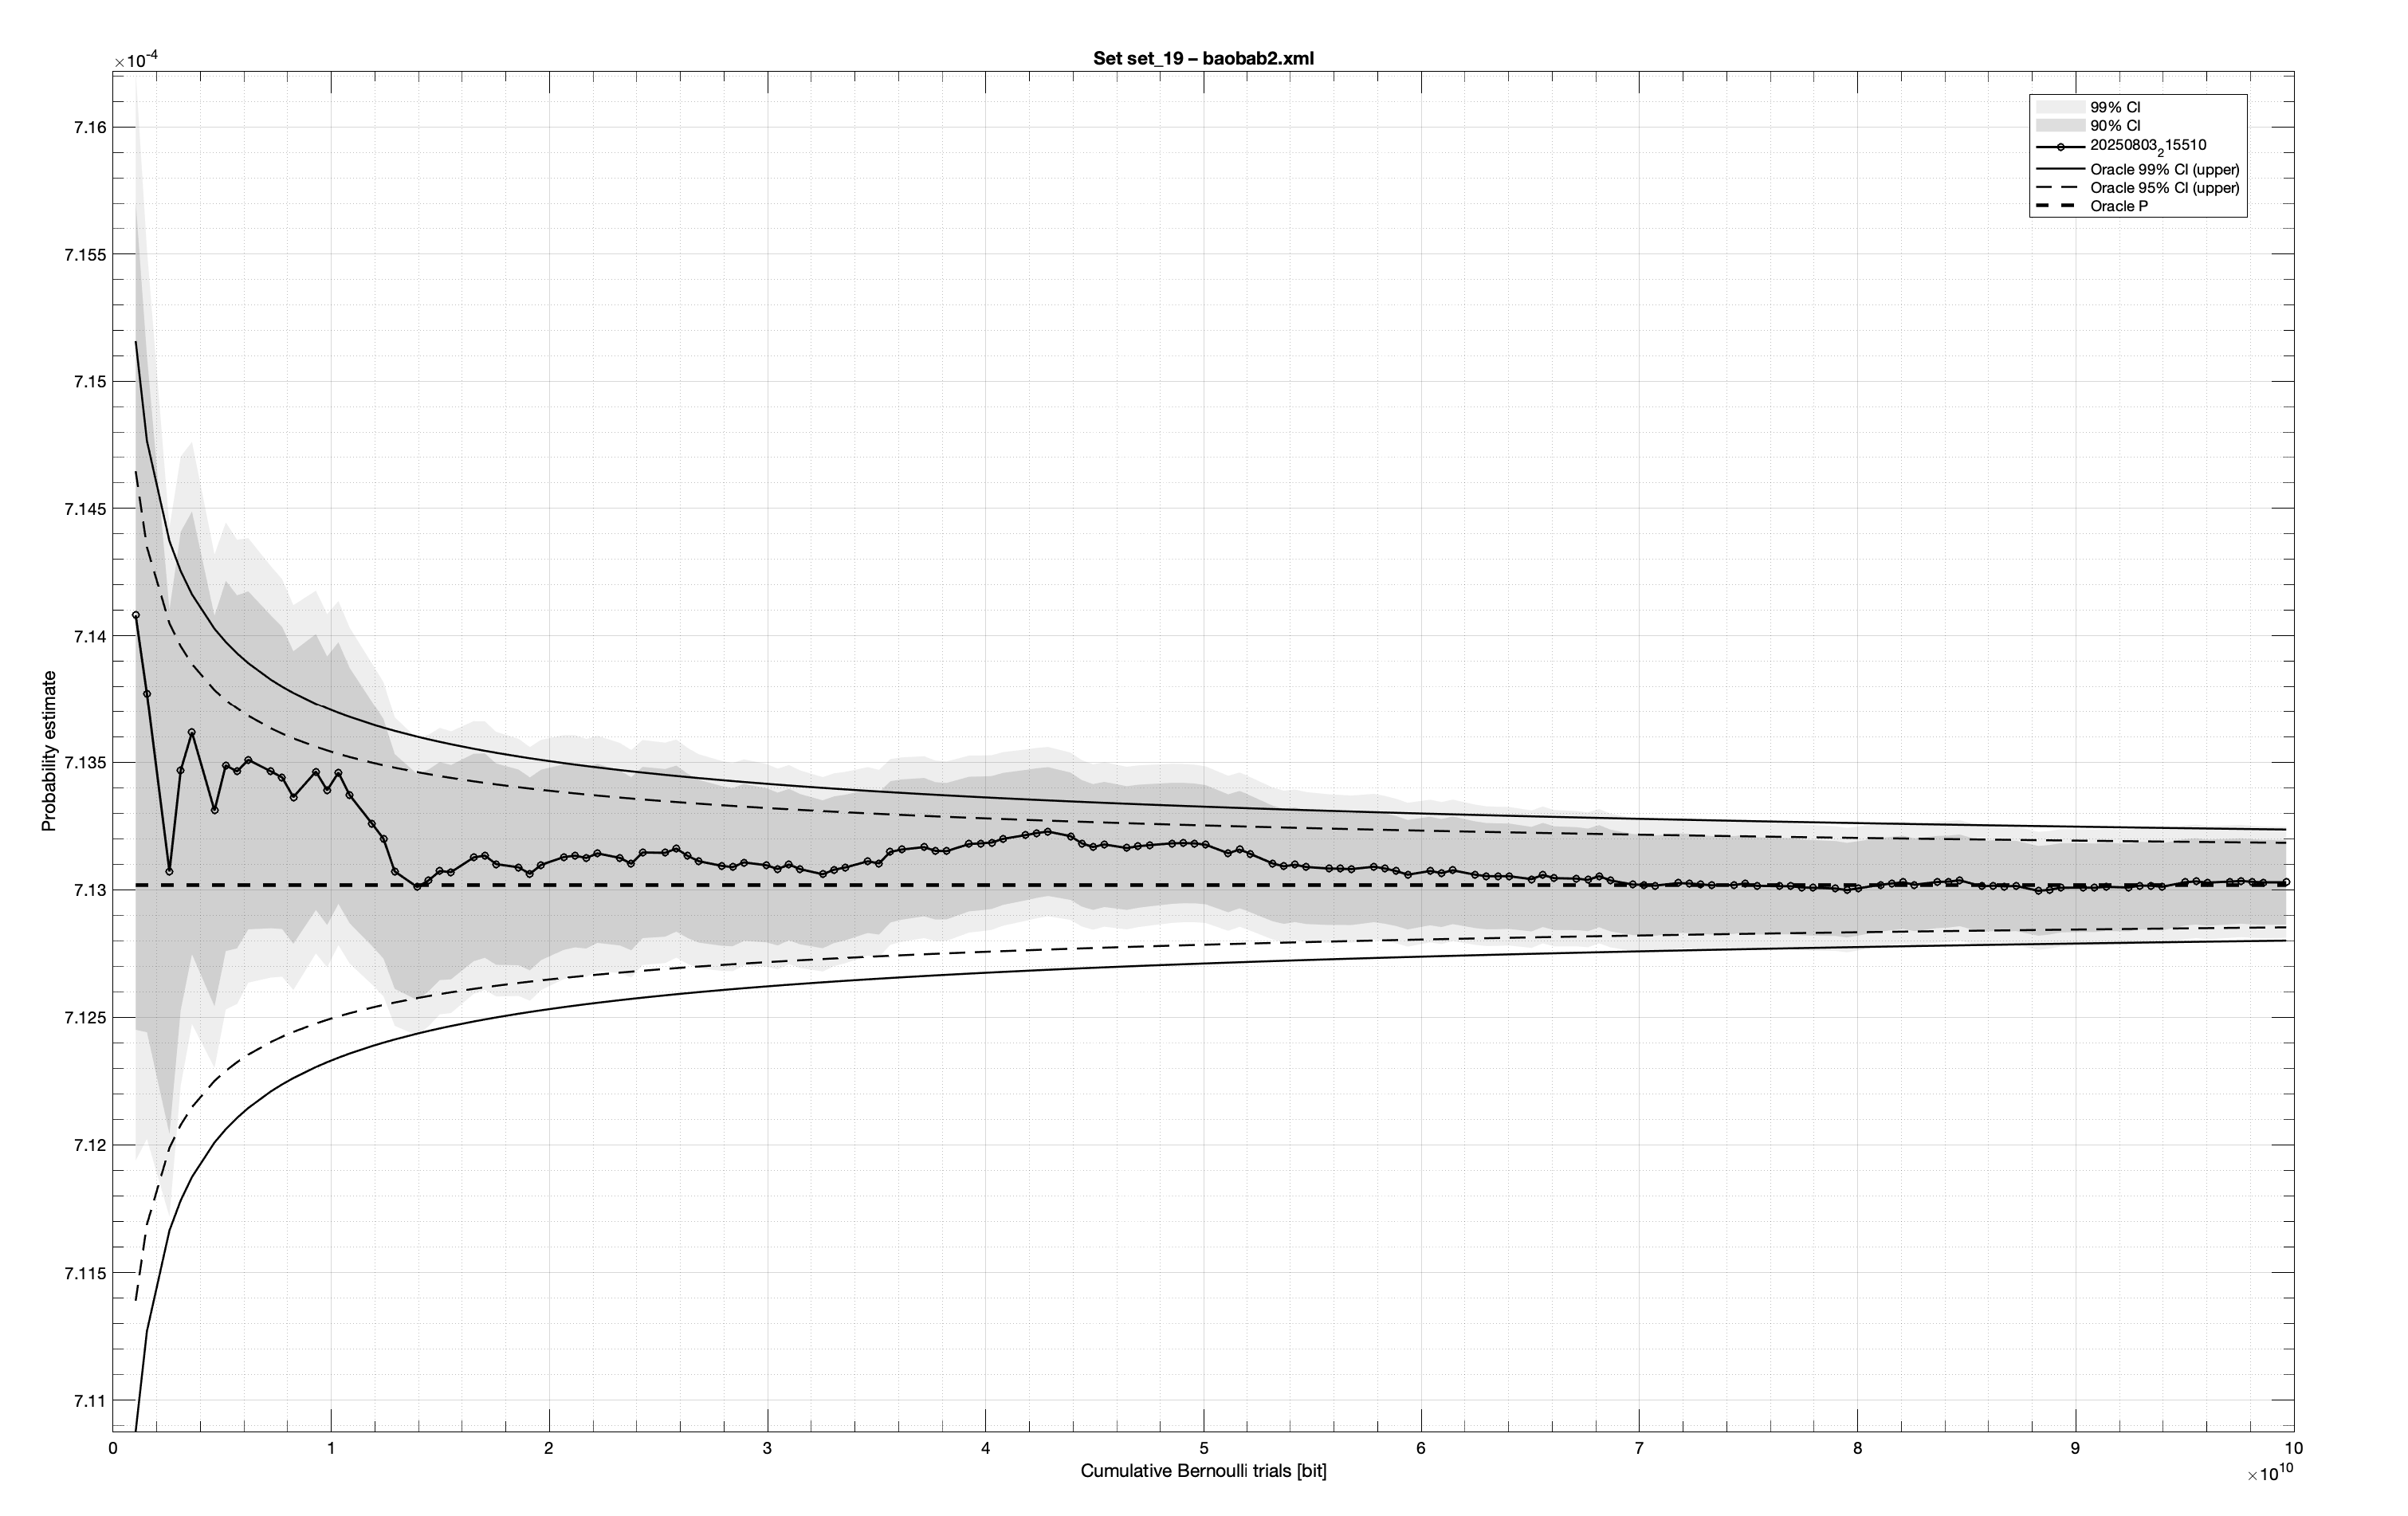
\includegraphics[width=0.95\linewidth]{2_framework/research_objective_3_mc_sampling/conv_fig_02.eps} % create trace: half-width vs iterations
      \vspace{-6pt}
  \end{columns}
\end{frame}